\documentclass[11pt,letterpaper]{article}
\usepackage[utf8]{inputenc}
\usepackage[top=1in,bottom=1in,left=1in,right=1in]{geometry}
\usepackage{amsmath}
\usepackage{amsfonts}
\usepackage{amssymb}
\usepackage{amsthm}
\usepackage{bm}
\usepackage{braket}
\usepackage{cancel}
\usepackage{enumitem}
\usepackage{float}
\usepackage{graphicx}
\usepackage{hyperref}
\usepackage{mathabx}
\usepackage{parskip}
\usepackage{tensor}
\usepackage{titlesec}
\usepackage{titling}
\usepackage{listings}




\titlelabel{(\thetitle)\quad}
\titleformat*{\section}{\large\bfseries}
\titleformat*{\subsection}{\normalsize\bfseries}
\setlength{\droptitle}{-5em}



\let\Re\relax
\DeclareMathOperator{\Re}{Re}
\let\Im\relax
\DeclareMathOperator{\Im}{Im}

\DeclareMathOperator*{\argmin}{arg\,min}
\DeclareMathOperator*{\argmax}{arg\,max}
\DeclareMathOperator*{\arginf}{arg\,inf}
\DeclareMathOperator*{\argsup}{arg\,sup}


\newcommand{\bhat}[1]{\hat{\bm{#1}}}


\renewcommand{\thesubsection}{\normalsize \alph{subsection}}
\renewcommand{\d}{\mathrm{d}}
\renewcommand{\vec}[1]{\bm{#1}}
\newcommand{\del}{\vec{\nabla}}
\newcommand{\e}{\epsilon}
\newcommand{\tpd}[3]{\left( \frac{\partial #1}{\partial #2} \right)_{#3}}
\newcommand{\pd}[2]{\frac{\partial #1}{\partial #2}}
\newcommand{\spd}[2]{\frac{\partial^2 #1}{\partial {#2}^2}}
\def\dbar{{\mathchar'26\mkern-12mu d}}

\allowdisplaybreaks


\author{Sam Kowash}
\numberwithin{equation}{section}
\numberwithin{figure}{section}
\title{CSE 546 HW \#2}

\begin{document}
\maketitle

{\bf Acknowledgments:} I collaborated on parts of this homework with Tyler Blanton, Michael Ross, and Nick Ruof.

\section{A Taste of Learning Theory}
\begin{enumerate}
	\item Let $X \in \mathbb{R}^d$ a random feature vector, and $Y \in \{1,\ldots,K\}$ a random label for $K\in \mathbb{N}$ with joint distribution $P_{XY}$. We consider a randomized classifier $\delta(x)$ which maps a value $x\in\mathbb{R}^d$ to some $y \in \{1,\ldots,K\}$ with probability $\alpha(x,y) \equiv P(\delta(x)=y)$ subject to $\sum_{y=1}^K \alpha(x,y) = 1$ for all $x$. The risk of the classifier $\delta$ is
	%
	\begin{align*}
		R(\delta) &\equiv \mathbb{E}_{XY,\delta}\left[\bm{1}\{\delta(X) \neq Y\}\right],
	\end{align*}
	%
	which we should interpret as the expected rate of misclassification. A classifier $\delta$ is called deterministic if $\alpha(x,y) \in \{0,1\}$ for all $x,y$. Further, we call a classifier $\delta_\ast$ a Bayes classifier if $\delta_\ast \in \arginf_\delta R(\delta)$.

	If we first take the expectation over outcomes of $\delta$ (by conditioning on $X$ and $Y$), we find
	%
	\begin{align*}
		R(\delta) &= \mathbb{E}_{XY}\left[1-\alpha(X,Y)\right],
	\end{align*}
	%
	since the indicator function is 1 except for the single outcome where $\delta(x)=y$, which occurs with probability $\alpha(x,y)$. It is then clear that minimizing $R(\delta)$ is equivalent to \emph{maximizing} $\mathbb{E}_{XY}[\alpha(X,Y)]$; the assignments of $\alpha(x,y)$ which do this are our Bayes optimal classifiers. 

















	\item Suppose we grab $n$ data samples $(x_i,y_i)$ i.i.d. from $P_{XY}$ where $y_i \in \{-1,1\}$ and $x_i \in \mathcal{X}$ where $\mathcal{X}$ is some set. Let $f: \mathcal{X} \to \{-1,1\}$ be a deterministic classifier with true risk
	%
	\begin{align*}
		R(f) &= \mathbb{E}_{XY}\left[\bm{1}(f(X) \neq Y)\right].
	\end{align*}
	%
	and empirical risk
	%
	\begin{align*}
		\hat{R}_n(f) &= \frac{1}{n} \sum_{i=1}^n \bm{1}(f(x_i) \neq y_i).
	\end{align*}




	\begin{enumerate}
		\item We wish to estimate the true risk of some classifier $\tilde{f}$. If we -
	\end{enumerate}

\end{enumerate}

























\section{Programming}
\begin{enumerate}
	\item 
		\begin{figure}[H]
			\centering
			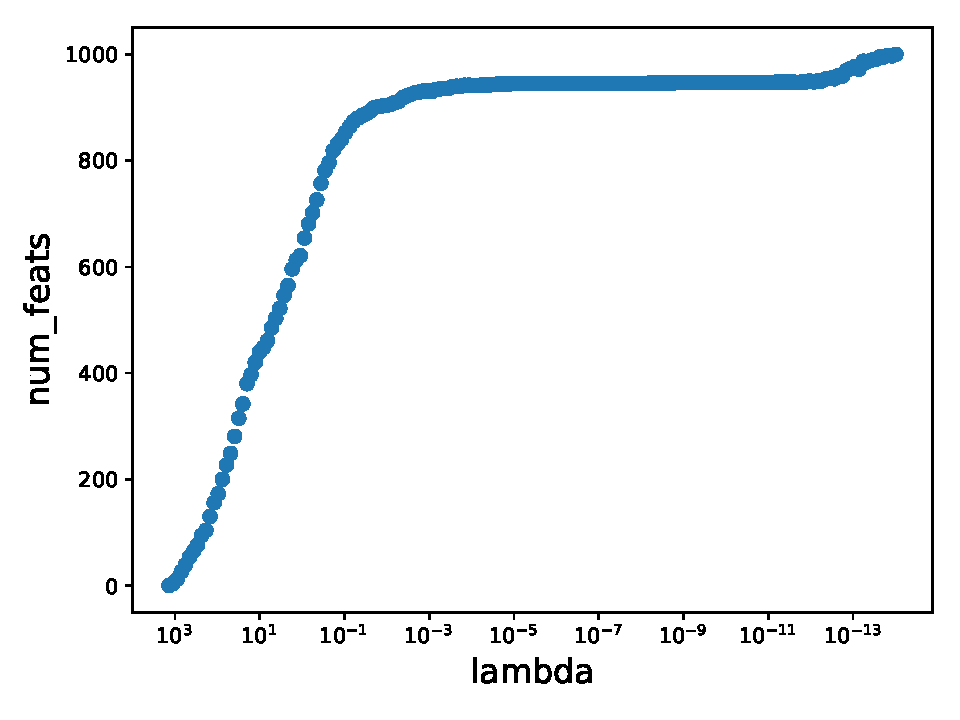
\includegraphics[width=0.6\textwidth]{figures/synth_nfeats_80.pdf}
			\caption{Number of nonzero features vs. $\lambda$ for lasso on synthetic data}
		\end{figure}

		\begin{figure}[H]
			\centering
			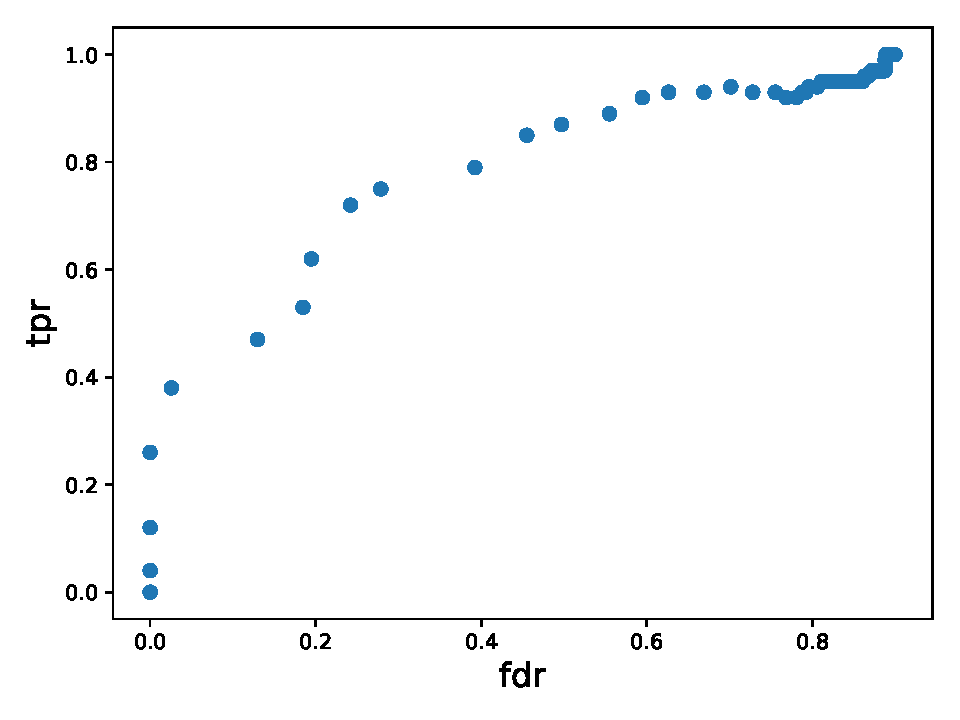
\includegraphics[width=0.6\textwidth]{figures/synth_fdr-tpr_80.pdf}
			\caption{TPR vs. FDR for lasso on synthetic data}-
		\end{figure}











	\item
	    

	Optimal $\lambda$ was near 1.11.
		\begin{figure}[H]
			\centering
			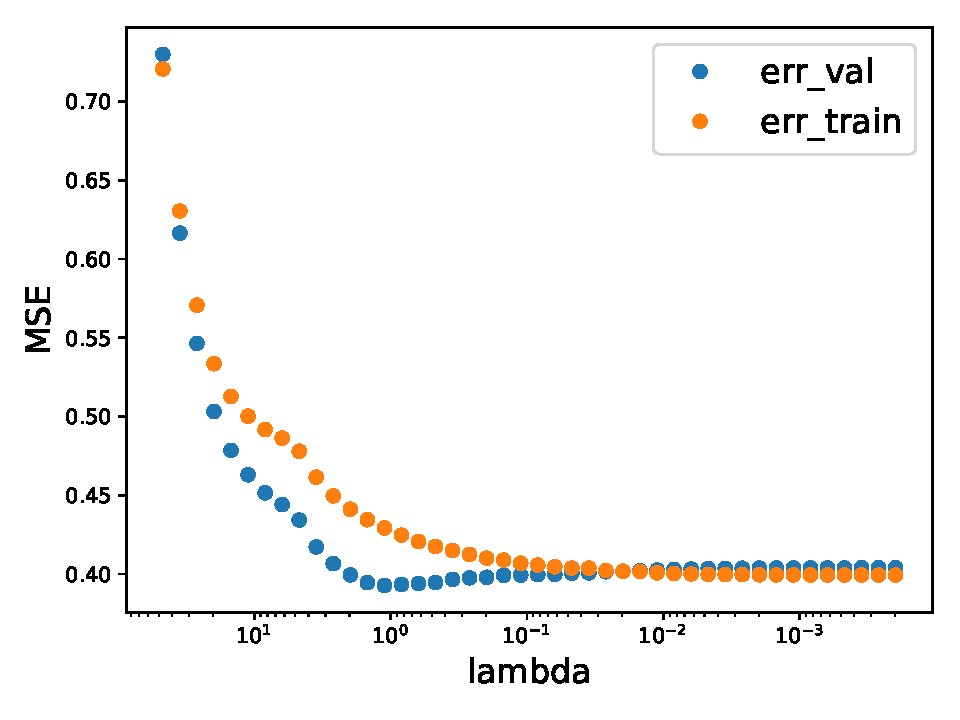
\includegraphics[width=.6\textwidth]{figures/yelp_errs.pdf}
			\caption{Validation and training error vs $\lambda$ on Yelp data}
		\end{figure}

		\begin{figure}[H]
			\centering
			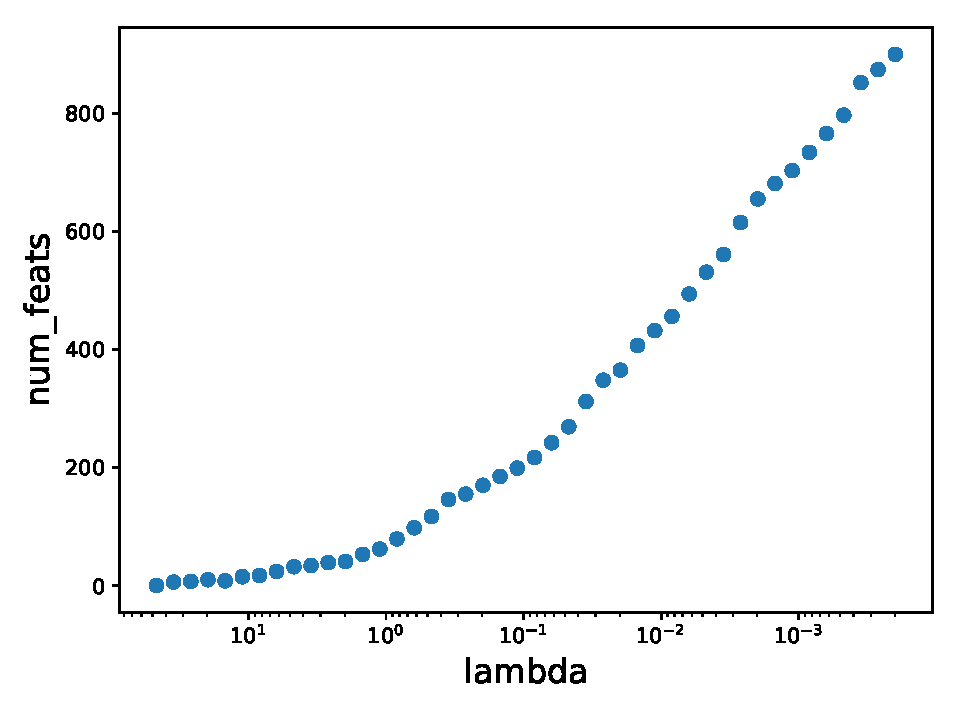
\includegraphics[width=.6\textwidth]{figures/yelp_nfeats.pdf}
			\caption{Number of nonzero features vs. $\lambda$ on Yelp data}
		\end{figure}















	\item We now consider binary classification between 2s and 7s in the MNIST set via regularized logistic regression. We choose a balanced target set $Y \in \{-1,1\}$, where $Y=-1$ for 2s and $Y = 1$ for 7s, so that our data are $\{(x_i,y_i)\}_{i=1}^n \subset \mathbb{R}^d \times \mathbb{Z}_2$. The $L_2$-regularized negative log likelihood objective to be minimized is
	%
	\begin{align*}
		J(w,b) &= \frac{1}{n} \sum_{i=1}^n \log\left[1 + \exp\left(-y_i(b+x_i^T w)\right)\right] + \lambda \|w\|_2^2.
	\end{align*}
	%
	For convenience, we define the functions
	%
	\begin{align*}
		\mu_i(w,b) &= \frac{1}{1+\exp\left[-y_i(b+x_i^T w)\right]}.
	\end{align*}.
	%
	\begin{enumerate}
		\item To do gradient descent, we need to know some gradients. First,
		\begin{align*}
			\nabla_w J(w,b) &= \frac{1}{n} \sum_{i=1}^n \frac{-y_i x_i \exp\left[-y_i(b + x_i^T w)\right]}{1 + \exp\left[-y_i(b+x_i^T w)\right]} + 2\lambda w\\
			\nabla_w J(w,b) &= -\frac{1}{n} \sum_{i=1}^n \mu_i \left(\frac{1}{\mu_i} - 1\right) y_i x_i + 2\lambda w\\
			\nabla_w J(w,b) &= \frac{1}{n} \sum_{i=1}^n (\mu_i - 1) y_i x_i + 2\lambda w.
		\end{align*}
		%
		Next,
		%
		\begin{align*}
			\nabla_b J(w,b) &= -\frac{1}{n} \sum_{i=1}^n \frac{y_i \exp\left[-y_i(b + x_i^T w)\right]}{1+\exp\left[-y_i(b+x_i^T w)\right]}\\
			\nabla_b J(w,b) &= \frac{1}{n} \sum_{i=1}^n (\mu_i -1) y_i.
		\end{align*}
		%
		We'll also want some Hessians, for Newton's method.
		%
		\begin{align*}
			\nabla^2_w J(w,b) &= \frac{1}{n} \sum_{i=1}^n y_i (\nabla_w \mu_i) x_i^T + 2\lambda I_d\\
			\nabla_w \mu_i &= \frac{y_i x_i \exp\left[-y_i(b+x_i^T w)\right]}{\left(1+\exp\left[-y_i(b+x_i^T w)\right]\right)^2} = \mu_i^2 \left(\frac{1}{\mu_i} - 1\right) y_i x_i = \mu_i (1- \mu_i) y_i x_i\\
			%
			\nabla^2_w J(w,b) &= \frac{1}{n} \sum_{i=1}^n \mu_i (1-\mu_i) y_i^2 x_i x_i^T + 2 \lambda I_d
		\end{align*}
		%
		Lastly,
		%
		\begin{align*}
			\nabla^2_b J(w,b) &= \frac{1}{n} \sum_{i=1}^n (\nabla_b \mu_i) y_i\\
			\nabla_b \mu_i &= \frac{y_i \exp\left[-y_i(b+x_i^T w)\right]}{\left(1+\exp\left[-y_i(b+x_i^T w)\right]\right)^2} = \mu_i(1-\mu_i)y_i\\
			\nabla^2_b J(w,b) &= \frac{1}{n} \sum_{i=1}^n \mu_i(1-\mu_i) y_i^2.
		\end{align*}
	\end{enumerate}
\end{enumerate}















\clearpage
\lstinputlisting[language=Python]{code/lasso.py}
\clearpage
\lstinputlisting[language=Python]{code/synth_lasso.py}
\clearpage
\lstinputlisting[language=Python]{code/yelp_lasso.py}
\clearpage
\lstinputlisting[language=Python]{code/grad_descend.py}



\end{document}